\documentclass[11pt,a4paper]{report}
\usepackage[textwidth=37em,vmargin=30mm]{geometry}
\usepackage{calc,xunicode,amsmath,amssymb,paralist,enumitem,tabu,booktabs,datetime2,xeCJK,xeCJKfntef,listings}
\usepackage{tocloft,fancyhdr,tcolorbox,xcolor,graphicx,eso-pic,xltxtra,xelatexemoji}

\newcommand{\envyear}[0]{2025}
\newcommand{\envdatestr}[0]{2025-07-11}
\newcommand{\envfinaldir}[0]{webdb/2025/20250711/final}

\usepackage[hidelinks]{hyperref}
\hypersetup{
    colorlinks=false,
    pdfpagemode=FullScreen,
    pdftitle={Web Digest - \envdatestr}
}

\setlength{\cftbeforechapskip}{10pt}
\renewcommand{\cftchapfont}{\rmfamily\bfseries\large\raggedright}
\setlength{\cftbeforesecskip}{2pt}
\renewcommand{\cftsecfont}{\sffamily\small\raggedright}

\setdefaultleftmargin{2em}{2em}{1em}{1em}{1em}{1em}

\usepackage{xeCJK,xeCJKfntef}
\xeCJKsetup{PunctStyle=plain,RubberPunctSkip=false,CJKglue=\strut\hskip 0pt plus 0.1em minus 0.05em,CJKecglue=\strut\hskip 0.22em plus 0.2em}
\XeTeXlinebreaklocale "zh"
\XeTeXlinebreakskip = 0pt


\setmainfont{Brygada 1918}
\setromanfont{Brygada 1918}
\setsansfont{IBM Plex Sans}
\setmonofont{JetBrains Mono NL}
\setCJKmainfont{Noto Serif CJK SC}
\setCJKromanfont{Noto Serif CJK SC}
\setCJKsansfont{Noto Sans CJK SC}
\setCJKmonofont{Noto Sans CJK SC}

\setlength{\parindent}{0pt}
\setlength{\parskip}{8pt}
\linespread{1.15}

\lstset{
	basicstyle=\ttfamily\footnotesize,
	numbersep=5pt,
	backgroundcolor=\color{black!5},
	showspaces=false,
	showstringspaces=false,
	showtabs=false,
	tabsize=2,
	captionpos=b,
	breaklines=true,
	breakatwhitespace=true,
	breakautoindent=true,
	linewidth=\textwidth
}






\newcommand{\coverpic}[2]{
    % argv: itemurl, authorname
    Cover photo by #2~~(\href{#1}{#1})
}
\newcommand{\makeheader}[0]{
    \begin{titlepage}
        % \newgeometry{hmargin=15mm,tmargin=21mm,bmargin=12mm}
        \begin{center}
            
            \rmfamily\scshape
            \fontspec{BaskervilleF}
            \fontspec{Old Standard}
            \fontsize{59pt}{70pt}\selectfont
            WEB\hfill DIGEST
            
            \vfill
            % \vskip 30pt
            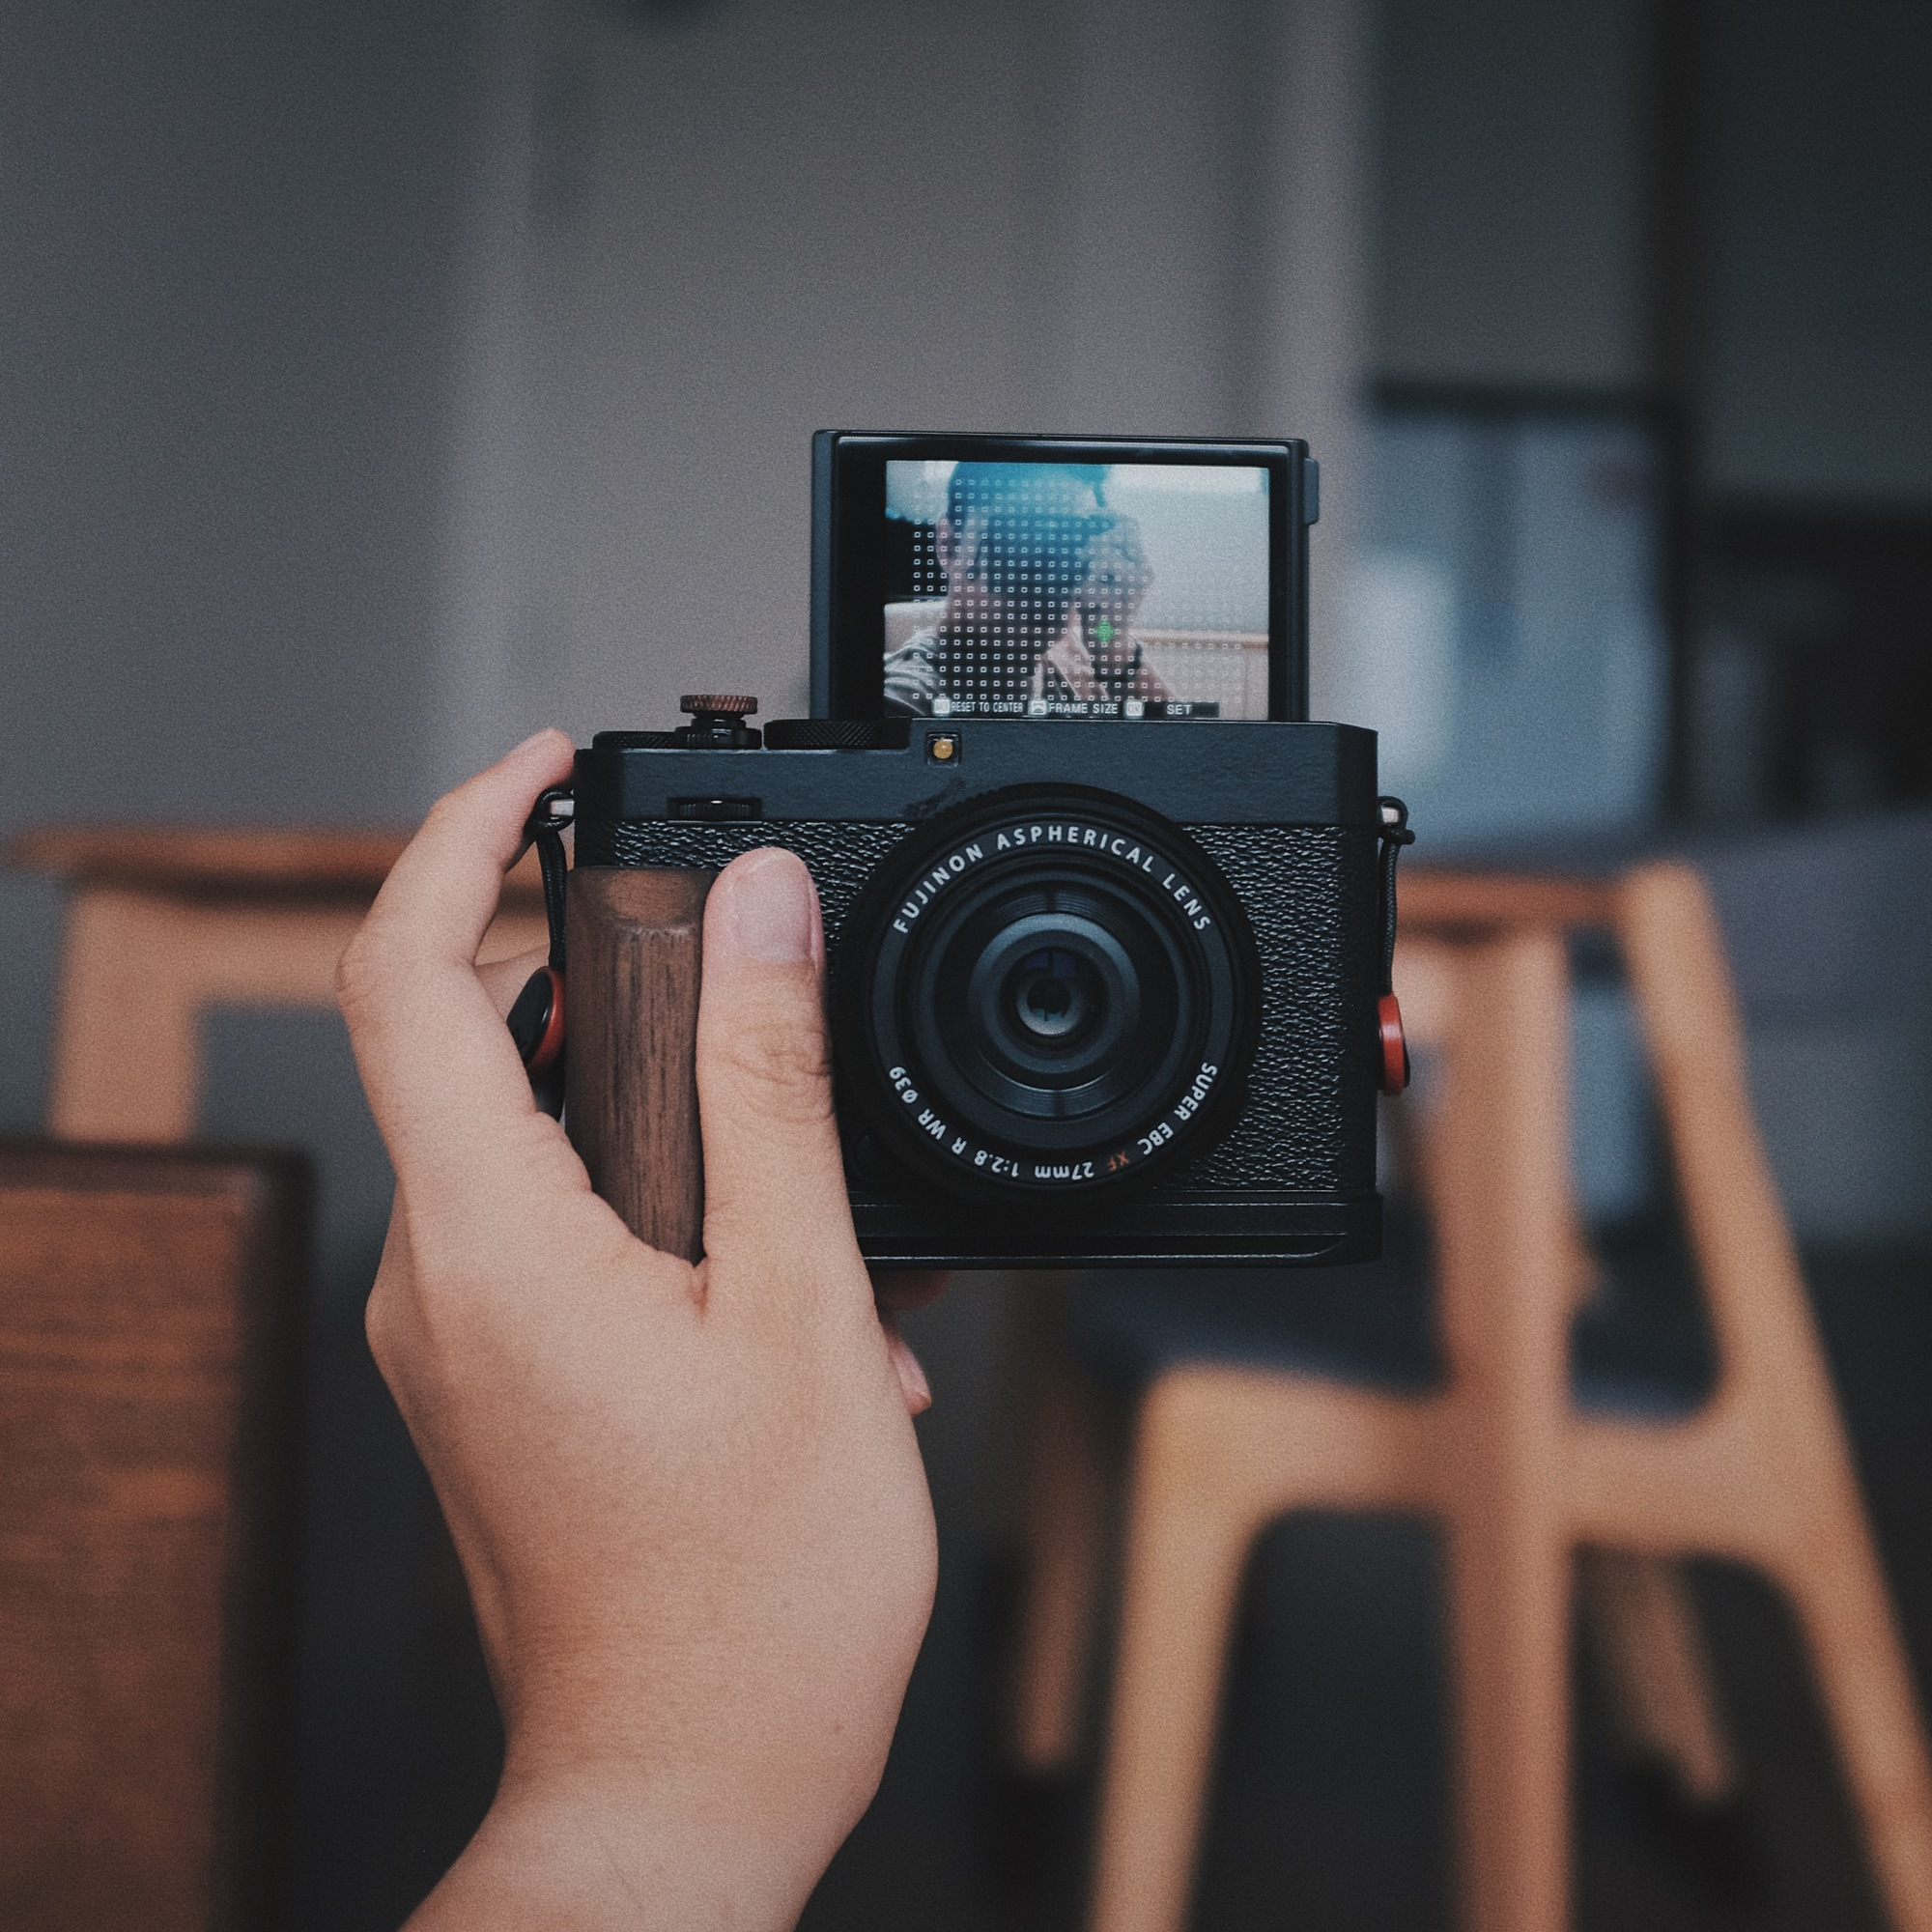
\includegraphics[width=\linewidth]{\envfinaldir/coverpic-prod.jpg}\par
            % \vskip 30pt
            \vfill

            \normalsize\rmfamily\scshape
            \copyright{} The Web Digest Project \hfill\large \envdatestr
        \end{center}
    \end{titlepage}
    % \restoregeometry
}
\newcommand{\simplehref}[1]{%
    \textcolor{blue!80!green}{\href{#1}{#1}}%
}
\renewcommand{\contentsname}{\center\Huge\sffamily\bfseries Contents\par\vskip 20pt}
\newcounter{ipartcounter}
\setcounter{ipartcounter}{0}
\newcommand{\ipart}[1]{
    % \vskip 20pt
    \clearpage
    \stepcounter{ipartcounter}
    \phantomsection
    \addcontentsline{toc}{chapter}{#1}
    % \begin{center}
    %     \Huge
    %     \sffamily\bfseries
    %     #1
    % \end{center}
    % \vskip 20pt plus 7pt
}
\newcounter{ichaptercounter}
\setcounter{ichaptercounter}{0}
\newcommand{\ichapter}[1]{
    % \vskip 20pt
    \clearpage
    \stepcounter{ichaptercounter}
    \phantomsection
    \addcontentsline{toc}{section}{\numberline{\arabic{ichaptercounter}}#1}
    \begin{center}
        \Huge
        \sffamily\bfseries
        #1
    \end{center}
    \vskip 20pt plus 7pt
}
\newcommand{\entrytitlefont}[1]{\subsection*{\raggedright\Large\sffamily\bfseries#1}}
\newcommand{\entryitemGeneric}[2]{
    % argv: title, url
    \parbox{\linewidth}{
        \entrytitlefont{#1}\par\vskip 5pt
        \footnotesize\ttfamily\mdseries
        \simplehref{#2}
    }\vskip 11pt plus 11pt minus 1pt
}
\newcommand{\entryitemGithub}[3]{
    % argv: title, url, desc
    \parbox{\linewidth}{
        \entrytitlefont{#1}\par\vskip 5pt
        \footnotesize\ttfamily\mdseries
        \simplehref{#2}\par\vskip 5pt
        \small\rmfamily\mdseries#3
    }\vskip 11pt plus 11pt minus 1pt
}
\newcommand{\entryitemAp}[3]{
    % argv: title, url, desc
    \parbox{\linewidth}{
        \entrytitlefont{#1}\par\vskip 5pt
        \footnotesize\ttfamily\mdseries
        \simplehref{#2}\par\vskip 5pt
        \small\rmfamily\mdseries#3
    }\vskip 11pt plus 11pt minus 1pt
}
\newcommand{\entryitemHackernews}[3]{
    % argv: title, hnurl, rawurl
    % \parbox{\linewidth}{
    %     \entrytitlefont{#1}\par\vskip 5pt
    %     \footnotesize\ttfamily\mdseries
    %     \simplehref{#3}\par
    %     \textcolor{black!50}{\href{#2}{#2}}
    % }\vskip 11pt plus 11pt minus 1pt
    \begin{minipage}{\linewidth}
            \entrytitlefont{#1}\par\vskip 5pt
            \footnotesize\ttfamily\mdseries
            \simplehref{#3}\par
            \textcolor{black!50}{\href{#2}{#2}}
    \end{minipage}\par\vskip 11pt plus 11pt minus 1pt
}







\begin{document}

\makeheader

\tableofcontents\clearpage




\ipart{Developers}
\ichapter{Hacker News}
\entryitemTwoLinks{Final report on Alaska Airlines Flight 1282 in-flight exit door plug separation}{https://news.ycombinator.com/item?id=44525468}{https://www.ntsb.gov:443/investigations/Pages/DCA24MA063.aspx}

\entryitemTwoLinks{Grok 4}{https://news.ycombinator.com/item?id=44524707}{https://simonwillison.net/2025/Jul/10/grok-4/}

\entryitemTwoLinks{Show HN: Open source alternative to Perplexity Comet}{https://news.ycombinator.com/item?id=44523409}{https://www.browseros.com/}

\entryitemTwoLinks{Measuring the impact of AI on experienced open-source developer productivity}{https://news.ycombinator.com/item?id=44522772}{https://metr.org/blog/2025-07-10-early-2025-ai-experienced-os-dev-study/}

\entryitemTwoLinks{Seven Engineers Suspended After \$2.3M Bridge Includes 90-Degree Turn}{https://news.ycombinator.com/item?id=44522579}{https://www.vice.com/en/article/7-engineers-suspended-after-2-3-million-bridge-includes-bizarre-90-degree-turn/}

\entryitemTwoLinks{Graphical Linear Algebra}{https://news.ycombinator.com/item?id=44522505}{https://graphicallinearalgebra.net/}

\entryitemTwoLinks{Bret Victor on why current trend of AIs is at odds with his work}{https://news.ycombinator.com/item?id=44522076}{https://dynamicland.org/2024/FAQ/\#What\_is\_Realtalks\_relationship\_to\_AI}

\entryitemTwoLinks{Red Hat Technical Writing Style Guide}{https://news.ycombinator.com/item?id=44521871}{https://stylepedia.net/style/}

\entryitemTwoLinks{Underwater turbine spinning for 6 years off Scotland's coast is a breakthrough}{https://news.ycombinator.com/item?id=44521457}{https://apnews.com/article/tidal-energy-turbine-marine-meygen-scotland-ffff3a7082205b33b612a1417e1ec6d6}

\entryitemTwoLinks{Flix – A powerful effect-oriented programming language}{https://news.ycombinator.com/item?id=44521224}{https://flix.dev/}

\entryitemTwoLinks{FOKS: Federated Open Key Service}{https://news.ycombinator.com/item?id=44520419}{https://foks.pub/}

\entryitemTwoLinks{Is Gemini 2.5 good at bounding boxes?}{https://news.ycombinator.com/item?id=44520292}{https://simedw.com/2025/07/10/gemini-bounding-boxes/}

\entryitemTwoLinks{How to prove false statements: Practical attacks on Fiat-Shamir}{https://news.ycombinator.com/item?id=44519175}{https://www.quantamagazine.org/computer-scientists-figure-out-how-to-prove-lies-20250709/}

\entryitemTwoLinks{Optimizing a Math Expression Parser in Rust}{https://news.ycombinator.com/item?id=44519034}{https://rpallas.xyz/math-parser/}

\entryitemTwoLinks{Show HN: Typeform was too expensive so I built my own forms}{https://news.ycombinator.com/item?id=44518898}{https://www.ikiform.com/}

\entryitemTwoLinks{Kite News}{https://news.ycombinator.com/item?id=44518473}{https://kite.kagi.com/}

\entryitemTwoLinks{Matt Trout has died}{https://news.ycombinator.com/item?id=44518269}{https://www.shadowcat.co.uk/2025/07/09/ripples-they-cause-in-the-world/}

\entryitemTwoLinks{German court rules Meta tracking technology violates European privacy laws}{https://news.ycombinator.com/item?id=44517424}{https://therecord.media/german-court-meta-tracking-tech}

\entryitemTwoLinks{Grok 4 Launch [video]}{https://news.ycombinator.com/item?id=44517055}{https://twitter.com/xai/status/1943158495588815072}

\entryitemTwoLinks{A Virginia public library is fighting off a takeover by private equity}{https://news.ycombinator.com/item?id=44516793}{https://lithub.com/a-virginia-public-library-is-fighting-off-a-threatened-takeover-by-private-equity/}


\ipart{Developers~~~~(zh-Hans)}
\ichapter{Solidot}
\entryitemGeneric{\hskip 0pt{}西欧经历有记录以来最热的六月}{https://www.solidot.org/story?sid=81764}

\entryitemGeneric{\hskip 0pt{}两性权力关系泾渭并不分明}{https://www.solidot.org/story?sid=81763}

\entryitemGeneric{\hskip 0pt{}OpenAI 将发布 AI Web 浏览器挑战 Chrome  }{https://www.solidot.org/story?sid=81762}

\entryitemGeneric{\hskip 0pt{}麦当劳的 AI 招聘平台管理员密码是 123456}{https://www.solidot.org/story?sid=81761}

\entryitemGeneric{\hskip 0pt{}英伟达市值突破 4 万亿美元}{https://www.solidot.org/story?sid=81760}

\entryitemGeneric{\hskip 0pt{}美国科技巨头对财政部的制裁名单响应并不迅速}{https://www.solidot.org/story?sid=81759}

\entryitemGeneric{\hskip 0pt{}一群抹香鲸被拍摄到以站立姿态睡觉}{https://www.solidot.org/story?sid=81758}

\entryitemGeneric{\hskip 0pt{}230 万 Chrome 和 Edge 用户安装了会劫持浏览器会话的扩展}{https://www.solidot.org/story?sid=81757}

\entryitemGeneric{\hskip 0pt{}研究估计未来的胃癌病例大部分与幽门螺杆菌感染相关}{https://www.solidot.org/story?sid=81756}

\entryitemGeneric{\hskip 0pt{}海马体在成年后仍然能生成新神经元}{https://www.solidot.org/story?sid=81755}

\entryitemGeneric{\hskip 0pt{}海法洞穴发现的古代骨骼可能是人类和尼安德特人混血}{https://www.solidot.org/story?sid=81754}

\entryitemGeneric{\hskip 0pt{}科学家首次直接观测到反Klein隧穿现象}{https://www.solidot.org/story?sid=81753}

\entryitemGeneric{\hskip 0pt{}TikTok 计划九月推出一个美国专用版本}{https://www.solidot.org/story?sid=81752}

\entryitemGeneric{\hskip 0pt{}开源工具帮助互联网抵御 AI 爬虫}{https://www.solidot.org/story?sid=81751}

\entryitemGeneric{\hskip 0pt{}Thunderbird 140 ESR 版释出}{https://www.solidot.org/story?sid=81750}

\entryitemGeneric{\hskip 0pt{}微软证书过期导致 Windows 7 更新出错}{https://www.solidot.org/story?sid=81749}

\entryitemGeneric{\hskip 0pt{}研究证实新质子幻数}{https://www.solidot.org/story?sid=81748}

\entryitemGeneric{\hskip 0pt{}NASA 新视野号成功演示深空恒星导航技术}{https://www.solidot.org/story?sid=81747}

\entryitemGeneric{\hskip 0pt{}日本生成式 AI 利用率 26\%}{https://www.solidot.org/story?sid=81746}

\entryitemGeneric{\hskip 0pt{}Netflix 称其全球订户有五成看动漫}{https://www.solidot.org/story?sid=81745}\ichapter{V2EX}
\entryitemGeneric{\hskip 0pt{}[程序员] 有什么内存/cpu 监控的小工具吗}{https://www.v2ex.com/t/1144432}

\entryitemGeneric{\hskip 0pt{}[Google] 一个手机号,辅助号码绑定(非注册),可以绑几个 Google 账号?}{https://www.v2ex.com/t/1144431}

\entryitemGeneric{\hskip 0pt{}[OpenAI] 大家一般倾向于用哪种文字(简体、繁体、英文……)向 chatgpt 或者其他 ai 工具提问呢?}{https://www.v2ex.com/t/1144430}

\entryitemGeneric{\hskip 0pt{}[阅读] 2025 六月读昆虫 蘑菇 罕见病 小说…… 12 本}{https://www.v2ex.com/t/1144429}

\entryitemGeneric{\hskip 0pt{}[互联网] 关于蜘蛛池,想请教几个菜鸟问题。}{https://www.v2ex.com/t/1144428}

\entryitemGeneric{\hskip 0pt{}[Android] 有用过一加手机的大佬吗,请教下耗电比较常快}{https://www.v2ex.com/t/1144427}

\entryitemGeneric{\hskip 0pt{}[程序员] 拆解飞书 AI:知识管理不可替代,多维表格意外突围}{https://www.v2ex.com/t/1144425}

\entryitemGeneric{\hskip 0pt{}[分享发现] 我用一套 AI 组合拳, 2 小时上线了一个产品验证页}{https://www.v2ex.com/t/1144423}

\entryitemGeneric{\hskip 0pt{}[PayPal] 现在美区 paypal 可以绑什么信用卡?}{https://www.v2ex.com/t/1144422}

\entryitemGeneric{\hskip 0pt{}[Ubuntu] 该装服务器了,装 Ubuntu24.04.2 还是 Ubuntu22.04.5}{https://www.v2ex.com/t/1144421}

\entryitemGeneric{\hskip 0pt{}[程序员] 多用户博客系统有推荐的吗}{https://www.v2ex.com/t/1144420}

\entryitemGeneric{\hskip 0pt{}[Android] 用外版手机在大陆入网 确定不是现眼包}{https://www.v2ex.com/t/1144419}

\entryitemGeneric{\hskip 0pt{}[问与答] 联通的套餐求推荐,哪个方案最合适我?}{https://www.v2ex.com/t/1144417}

\entryitemGeneric{\hskip 0pt{}[问与答] siri 如何呼唤出来 原生的 apple music}{https://www.v2ex.com/t/1144416}

\entryitemGeneric{\hskip 0pt{}[Apple] 苹果的 [密码] APP 一天要输入 N 次密码解锁}{https://www.v2ex.com/t/1144415}

\entryitemGeneric{\hskip 0pt{}[生活] 来自一个京东外卖众包的吐槽!~}{https://www.v2ex.com/t/1144414}

\entryitemGeneric{\hskip 0pt{}[Claude] Claude Code vs Cursor 你们觉得哪个更好用}{https://www.v2ex.com/t/1144413}

\entryitemGeneric{\hskip 0pt{}[问与答] 有支持 OPPO 推送到邮件 app 吗}{https://www.v2ex.com/t/1144412}

\entryitemGeneric{\hskip 0pt{}[问与答] HR 小调研:如果没周年有一次薪资回顾,你认为重要吗?}{https://www.v2ex.com/t/1144411}

\entryitemGeneric{\hskip 0pt{}[问与答] 当前最佳的 Minio 替代品是什么?}{https://www.v2ex.com/t/1144410}

\entryitemGeneric{\hskip 0pt{}[分享创造] 介绍一个无聊但是能提高工作效率的网站——ExtractAny}{https://www.v2ex.com/t/1144408}

\entryitemGeneric{\hskip 0pt{}[加密货币] 2025 年 7 月,中国大陆居民如何尽可能合法且方便的获取并使用虚拟币?}{https://www.v2ex.com/t/1144407}

\entryitemGeneric{\hskip 0pt{}[Telegram] 接码平台推荐,注册 Telegram 与其他 APP 海外号码}{https://www.v2ex.com/t/1144405}

\entryitemGeneric{\hskip 0pt{}[加密货币] 有哪些偏正经的商品或服务,是可以用数字货币购买/订阅的?}{https://www.v2ex.com/t/1144404}

\entryitemGeneric{\hskip 0pt{}[程序员] 关于免费 Windows Electron 桌面小程序签名的问题}{https://www.v2ex.com/t/1144403}

\entryitemGeneric{\hskip 0pt{}[远程工作] [帮发] AI 应用创业团队招全栈 / 前端 / 后端 / AI 工程师(React + Node.js + AI)}{https://www.v2ex.com/t/1144401}

\entryitemGeneric{\hskip 0pt{}[程序员] 千万不要去试用 iOS Shortcut 自动打卡…}{https://www.v2ex.com/t/1144400}

\entryitemGeneric{\hskip 0pt{}[投资] 2025 年已过半,截至目前,今年你的股票/期货或者其他权益资产收益怎么样?}{https://www.v2ex.com/t/1144399}

\entryitemGeneric{\hskip 0pt{}[VPS] 240 收一台 NC rs2000 g9.5 美东 9634}{https://www.v2ex.com/t/1144398}

\entryitemGeneric{\hskip 0pt{}[DNS] 分享一个自建 dns}{https://www.v2ex.com/t/1144397}

\entryitemGeneric{\hskip 0pt{}[Apple] 发现从 iPhone 15 系列开始, iPhone 的电池变得极其耐用(以及 Apple care 澳门维修的流程请教)}{https://www.v2ex.com/t/1144396}

\entryitemGeneric{\hskip 0pt{}[V2EX] 关于 QQ 邮箱的问题}{https://www.v2ex.com/t/1144393}

\entryitemGeneric{\hskip 0pt{}[科幻] 以后内容由 AI 生成之后, 那信息是会更好还是更坏?}{https://www.v2ex.com/t/1144392}

\entryitemGeneric{\hskip 0pt{}[问与答] 怀疑显示器和线材的问题}{https://www.v2ex.com/t/1144390}

\entryitemGeneric{\hskip 0pt{}[程序员] 使用 Claude Code 中转商的风险}{https://www.v2ex.com/t/1144388}

\entryitemGeneric{\hskip 0pt{}[分享创造] 真开源跨平台电子书阅读软件 Readest,即将发布正式版本 1.0}{https://www.v2ex.com/t/1144387}

\entryitemGeneric{\hskip 0pt{}[分享发现] 云贵川有高性价比的数字游民社区吗}{https://www.v2ex.com/t/1144385}

\entryitemGeneric{\hskip 0pt{}[问与答] 请教一下大佬们,软件加急有用吗?}{https://www.v2ex.com/t/1144384}

\entryitemGeneric{\hskip 0pt{}[酷工作] [社招] [组内直招] [滴滴] [北京] 工程推荐搜索方向}{https://www.v2ex.com/t/1144382}

\entryitemGeneric{\hskip 0pt{}[Python] 如何使用程序识别视频里面是否含有水印、字幕?}{https://www.v2ex.com/t/1144381}

\entryitemGeneric{\hskip 0pt{}[酷工作] [北京] 头部电网公司电力人工智能调度系统招聘前端、后端}{https://www.v2ex.com/t/1144379}

\entryitemGeneric{\hskip 0pt{}[分享发现] Drizzle ORM:轻量级数据库工具}{https://www.v2ex.com/t/1144378}

\entryitemGeneric{\hskip 0pt{}[全球工单系统] 微软的 ToDo 今天是挂了吗?}{https://www.v2ex.com/t/1144377}

\entryitemGeneric{\hskip 0pt{}[问与答] Outlook 是不是崩了?}{https://www.v2ex.com/t/1144376}

\entryitemGeneric{\hskip 0pt{}[问与答] 现在想买一台 75 寸的电视机,有什么性价比高的电视机品牌推荐吗?}{https://www.v2ex.com/t/1144375}

\entryitemGeneric{\hskip 0pt{}[职场话题] 公司倒闭,帮同事做背调,对方只关心有没有劳务仲裁}{https://www.v2ex.com/t/1144374}

\entryitemGeneric{\hskip 0pt{}[Google] 使用 谷歌账号授权登录的 V2EX, 怎么设置密码?}{https://www.v2ex.com/t/1144373}

\entryitemGeneric{\hskip 0pt{}[分享发现] 我的第二个全栈开发项目:吃啥好呢 - 个性化美食推荐}{https://www.v2ex.com/t/1144372}

\entryitemGeneric{\hskip 0pt{}[健身] 这是一个产品经理转型自由教练的故事}{https://www.v2ex.com/t/1144371}

\entryitemGeneric{\hskip 0pt{}[投资] 想拿点钱做一些有波动的投资, A 股还是虚拟币?}{https://www.v2ex.com/t/1144369}


\ipart{Generic News}







\clearpage
\leavevmode\vfill
\footnotesize

Copyright \copyright{} 2023-2025 Neruthes and other contributors.

This document is published with CC BY-NC-ND 4.0 license.

The entries listed in this newsletter may be copyrighted by their respective creators.

This newsletter is generated by the Web Digest project.

The newsletters are also delivered via Telegram channel \CJKunderline{\href{https://t.me/webdigestchannel}{https://t.me/webdigestchannel}}.\\
RSS feed is available at \CJKunderline{\href{https://webdigest.pages.dev/rss.xml}{https://webdigest.pages.dev/rss.xml}}.

This newsletter is available in PDF at
\CJKunderline{\href{https://webdigest.pages.dev/}{https://webdigest.pages.dev/}}.

The source code being used to generate this newsletter is available at\\
\CJKunderline{\href{https://github.com/neruthes/webdigest}{https://github.com/neruthes/webdigest}}.

This newsletter is also available in
\CJKunderline{\href{http://webdigest.pages.dev/readhtml/\envyear/WebDigest-20250711.html}{HTML}} and
\CJKunderline{\href{https://github.com/neruthes/webdigest/blob/master/markdown/\envyear/WebDigest-20250711.md}{Markdown}}.


\coverpic{https://unsplash.com/photos/cherry-blossoms-hang-gracefully-against-a-dark-background-GGCYBMYu7a0}{Eric Soubeyrand}


\end{document}
